% !TEX root = ../Thesis.tex
%
%\documentclass{article}
%\usepackage{graphicx,tikz}
%\usepackage[graphics,tightpage,active]{preview}
%\PreviewEnvironment{tikzpicture}
%\begin{document}
%%%%%%%%%%%%%%%%%%%%%%%%%%%%%%%%%%%%%%%%%%%%%%%%%
	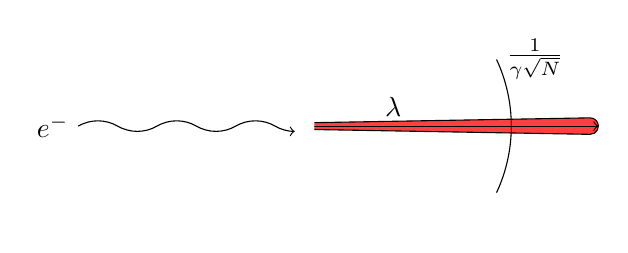
\begin{tikzpicture}
		%\draw [help lines] (0,0) grid (5,5);
		\def\a{120}	% 90+40
		\def\b{60}		% 90-40 
		\def\c{-120}
		\def\d{-60}
		\def\length{0.5}
		\def\start{-.5}
		% travelling electron
			\node [anchor=east] at (\start,0) {$e^{-}$};
			\draw [->] (\start,0) arc (\a:\b:\length) arc (\c:\d:\length) arc (\a:\b:\length) arc (\c:\d:\length) arc (\a:\b:\length) arc (\c:-90:\length);
		% beam angle
		\clip (2.5,-1.25) rectangle (6.125,1.25);
			\draw (5,0) arc (0:-25:2);
			\draw (5,0) arc (0:25:2) node [right] {$\frac{1}{\gamma\sqrt{N}}$};
		% beam
			\def\alpha{1}
			\def\length{6}
			\def\arclength{0.10473038956930551459077337131837} % arclength = tan(\alpha)*\length
			\fill [color=red,nearly opaque] (0,0) -- (\alpha:\length) arc (90+\alpha:-90-\alpha:\arclength) -- cycle; 
			\draw (\alpha:\length) arc (90+\alpha:-90-\alpha:\arclength);
			\node at (3.5,.25) {$\lambda$};
		% arrows
			\draw (0,0) -- (\alpha:\length);
			\draw [->] (0,0) -- (\length+\arclength,0);
			\draw (0,0) -- (-\alpha:\length);
	\end{tikzpicture}
%%%%%%%%%%%%%%%%%%%%%%%%%%%%%%%%%%%%%%%%%%%%%%%%%
%\end{document}